\documentclass[a4paper,11pt]{report}


%%%%  The next package provides very powerful methods for 
%%%%  drawing figures, but be warned that the manual for the 
%%%%  package is 400 pages long.  
\usepackage{tikz}


%%%%  Add some length to the page, as margins always seem too big.  
\addtolength{\topmargin}{-1.5in}
\addtolength{\textheight}{2in}

\begin{document}

%%%%  Number the initial front matter with roman numerals
\pagenumbering{roman}


%%%%  TITLE PAGE
%%  Here are the elements that make up the title page of the document.  

\thispagestyle{empty}  %%  Make the title page have no number.  

%%%%  INSERT TITLE AND NAME HERE!!
\title{\LARGE
The Dissertation Title}

\author{Your name here
\\    \\    \\
A DISSERTATION
\\    \\
Submitted to 
\\    \\    \\ 
The University of Liverpool
\\    \\
\\    \\
in partial fulfilment of the requirements
\\
for the degree of 
\\     \\
MASTER OF SCIENCE
\\     \\    \\    \\
}


%%  Fill in a date here if you want, or comment out the line below and
%%  the current date will be automatically inserted for you.  
\date{}


\maketitle


%%%%  ABSTRACT
\chapter*{\center Abstract}

Provide some brief description of your project, what the goals were,
what experiments were to be performed, what software was
to be developed, what was accomplished in the project, etc.  

This should provide some overview that could generally 
be understood by a 
non-specialist.  

\newpage



%%%%  STUDENT DECLARATION ON PLAGIARISM
\chapter*{\center Student Declaration} 

I confirm that I have read and understood the University's Academic Integrity Policy.

I confirm that I have acted honestly, ethically and professionally in conduct leading
to assessment for the programme of study.  

I confirm that I have not copied material from another source nor committed plagiarism
nor fabricated data when completing the attached piece of work.  I confirm that I have 
not previously presented the work or part thereof for assessment for another University
of Liverpool module.  I confirm that I have not copied material from another source, nor
colluded with any other student in the preparation and production of this work.  

I confirm that I have not incorporated into this assignment material that has been 
submitted by me or any other person in support of a successful application for a 
degree of this or any other university or degree-awarding body.  

\vspace*{1in}

\noindent SIGNATURE \verb!______________________________________!

\noindent DATE \hspace*{.4in}  \today

\vspace*{1in}

%%  NOTE ABOUT CONFIDENTIAL MATERIAL  
%%     Students who need to keep their dissertation confidential should uncomment
%%     the following sentence on this same page.  This will preclude the dissertation 
%%     from being placed in the University Library.  Students that submit work that 
%%     isn't confidential should leave this line commented out.  

% This dissertation contains material that is confidential and/or commercially
% sensitive. It is included here on the understanding that this will not be revealed to 
% any person not involved in the assessment process.  


\newpage

%%%%  ACKNOWLEDGMENTS
%%%%    A section for Acknowledgments, should you want one.

\chapter*{\center Acknowledgments}

XXXXXXXXXXXXXXXXXXXXXXXXXXXXXXXXXXXXXX

\noindent XXXXXXXXXXXXXXXXXXXXXXXXXXXXXXXXXXXXXX


\newpage


%%%%  TABLE OF CONTENTS  
%%%%      Usually the following command will give you the formatting you want.  

\tableofcontents



%%%%  LIST OF FIGURES
%%%%      Comment out this line if you have no figures in your document.  
\listoffigures


%%%%  LIST OF TABLES  
%%%%      Comment out this next line if you have no tables in your document.  
\listoftables



\newpage


%%%%  Turn page numbering back to arabic.  This also resets the numbering
%%%%  to begin again at page 1.  

\pagenumbering{arabic}

%%%%  INTRODUCTION

\chapter{Introduction}\label{chap:intro}
 
This project describes the greatest invention since sliced bread, 
namely twice-sliced bread.  


\section{Scope}

\section{Problem Statement}\label{sec:problem}

\section{Approach}

See Fig.~\ref{fig:first} for a nice pretty picture that I have included
in my dissertation.  


\section {Outcome}



%%%%  BACKGROUND

\chapter{Background}\label{chap:background}

We base some of our results on the previous work of other authors~\cite{A1, Someone}.


%%%%  DESIGN

\chapter{Design}\label{chap:design}

In this chapter, we will outline the design of the software that was
developed in this project.  

\section{Original design}\label{chap:first_design}
The original design document that was submitted can be found in 
Appendix~\ref{app:Original_design}.  The idea of that design
was as follows....


\section{Changes to original design}


%%%%  IMPLEMENTATION

\chapter{Implementation}\label{chap:implementation}


%%%%  This figure uses the "tikz" package mentioned earlier to
%%%%  draw it.  Obviously there are other ways to draw pictures,
%%%%  including native LaTeX commands for doing so.  I am merely
%%%%  providing an example here.  The "label" is how you can 
%%%%  add a label to refer to the figure in the body of the document.
\begin{figure}[ht]
  \caption{A pretty picture to add something to my dissertation}
\label{fig:first}
\centering

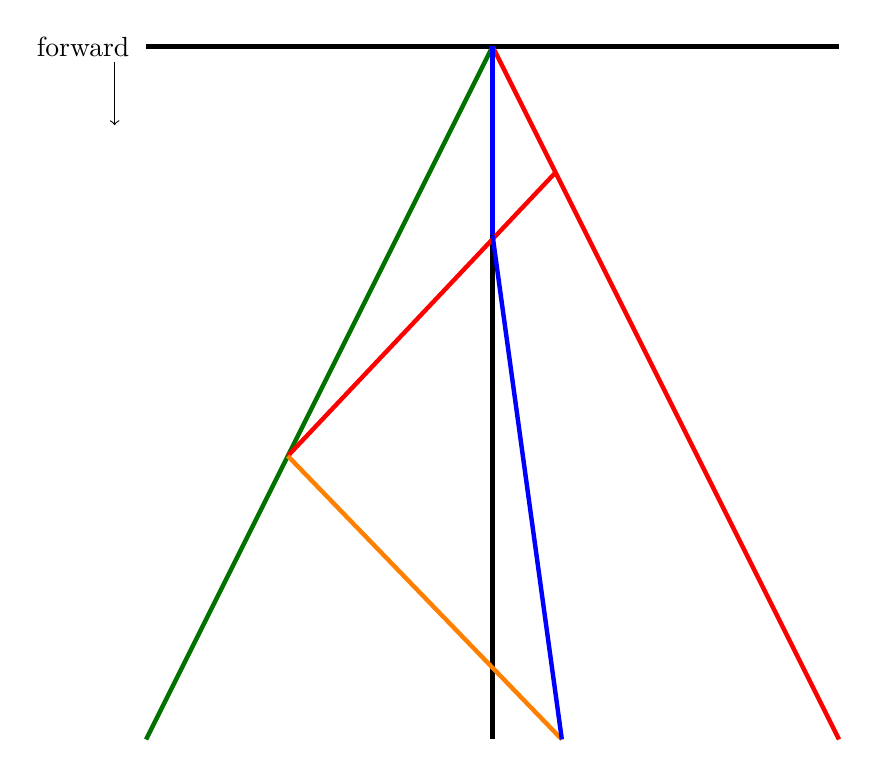
\begin{tikzpicture}[scale=0.4]

\path (6,14) coordinate (origin);
\path (17,14) coordinate (P0);
\path (-5,14) coordinate (P1);
\path (6,-8) coordinate (P2);

\path (5.5,13.5) coordinate (RedT1);
\path (7,12) coordinate (RedT2);
\path (4,9) coordinate (RedT3);
\path (10,3) coordinate (RedT4);
\path (17,-8) coordinate (RedEnd);

\path (5.5,13.5) coordinate (GreenT1);
\path (7,12) coordinate (GreenT2);
\path (4,9) coordinate (GreenT3);
\path (10,3) coordinate (GreenT4);
\path (-5,-8) coordinate (GreenEnd);

\path (8,14) coordinate (P5);
\path (8,10) coordinate (P6);
\path (6,8) coordinate (P7);
\path (-0.5,1) coordinate (P8);
\path (8.15,-3) coordinate (P9);
\path (8.2,-8) coordinate (P10);

\path (6,1) coordinate (BlueT1);

\draw [black,ultra thick] (P0) -- (P1);
\draw [black,ultra thick] (origin) -- (P2);
\draw [red,ultra thick] (origin) -- (RedEnd);
\draw [green!45!black,ultra thick] (origin) -- (GreenEnd);
\draw [blue,ultra thick] (origin) -- (P7);

\draw [red, ultra thick] (P6) -- (P8);
\draw [orange, ultra thick] (P8) -- (P10);

\draw [blue, ultra thick] (P7) -- (P10);

\draw (-7,14) node {forward};
\draw [->] (-6,13.5) -- (-6,11.5); 
\end{tikzpicture}
\end{figure} 



%%%%   REFERENCES

%%%%  Section for references, using the \bibitem directive to 
%%%%  specify labels used to cite sources in the document.  

\begin{thebibliography}{99}
\addcontentsline{toc}{chapter}{Bibliography}

\bibitem{A1}
A.N.~Author.  The best paper of all.
{\em Some really good reference} {\bf 12}, pp.~100--113, 2003.

\bibitem{Someone}
S.~omeone.  A paper that I wish I'd written.  
{\em J.\ Combinatorics} {\bf 34}, pp.~25--78, 1979.  

\end{thebibliography}


%%%%   APPENDICES
\appendix

%%%  First appendix.  

\chapter{Some Interesting Bit of Code}\label{app:Code}

I might include some particularly interesting part of my code here that is
referred to elsewhere in the document.  



%%%  A second appendix.

\chapter{Experimental results}\label{app:Experiments}

Here I give details of some experiments that were performed during the
course of the project.  

%%%
\section{Experiment 1}

Some stuff here.  


%%%
\section{Experiment 2}

Some more stuff here.


%%%  Original design document.
\chapter{Original design document}\label{app:Original_design}

Here I might insert the original design document for the project, in order
to refer to it and changes that I made.  

\end{document}
